\section*{Anhang}\label{sec:anhang}
\begin{figure}[H]
	\centering
	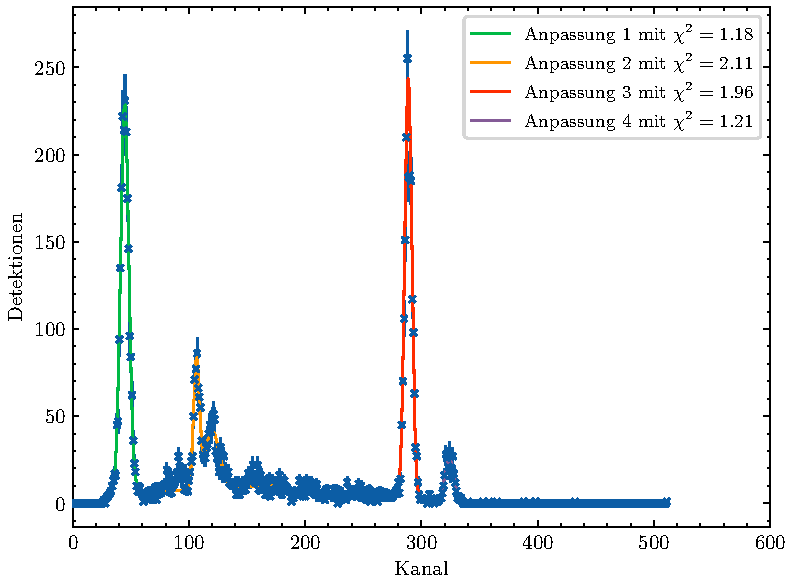
\includegraphics[width=0.6\linewidth]{../figs/Ag.pdf}
	\caption{Referenzspektrum für Silber.}
	\label{fig:ag}
\end{figure}
\begin{figure}[H]
	\centering
	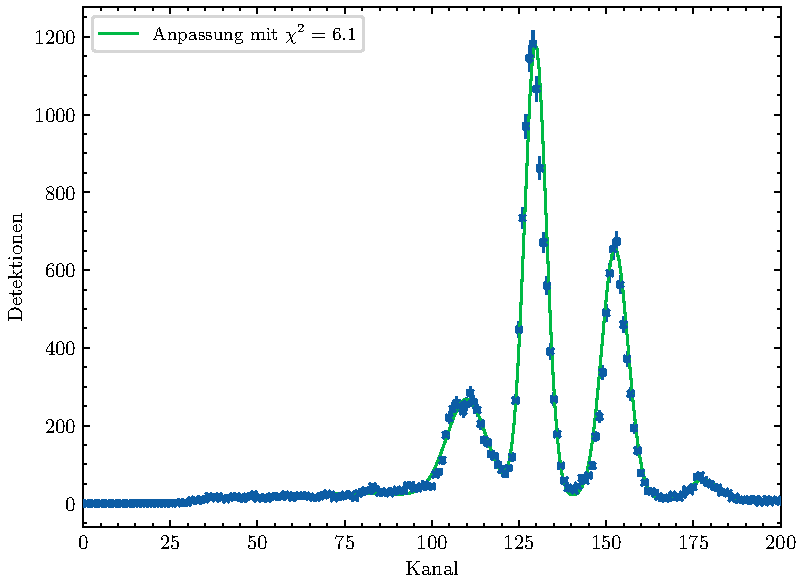
\includegraphics[width=0.6\linewidth]{../figs/Au.pdf}
	\caption{Referenzspektrum für Gold.}
	\label{fig:au}
\end{figure}
\begin{figure}[H]
	\centering
	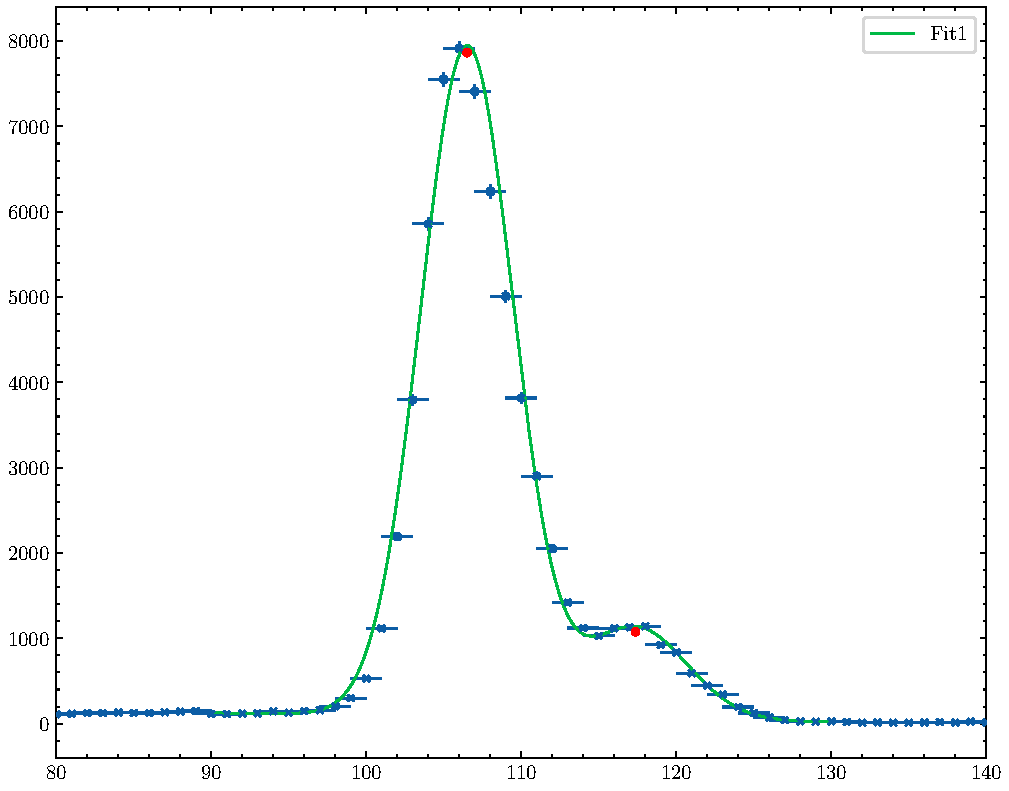
\includegraphics[width=0.6\linewidth]{../figs/Cu.pdf}
	\caption{Referenzspektrum für Kupfer.}
	\label{fig:cu}
\end{figure}
\begin{figure}[H]
	\centering
	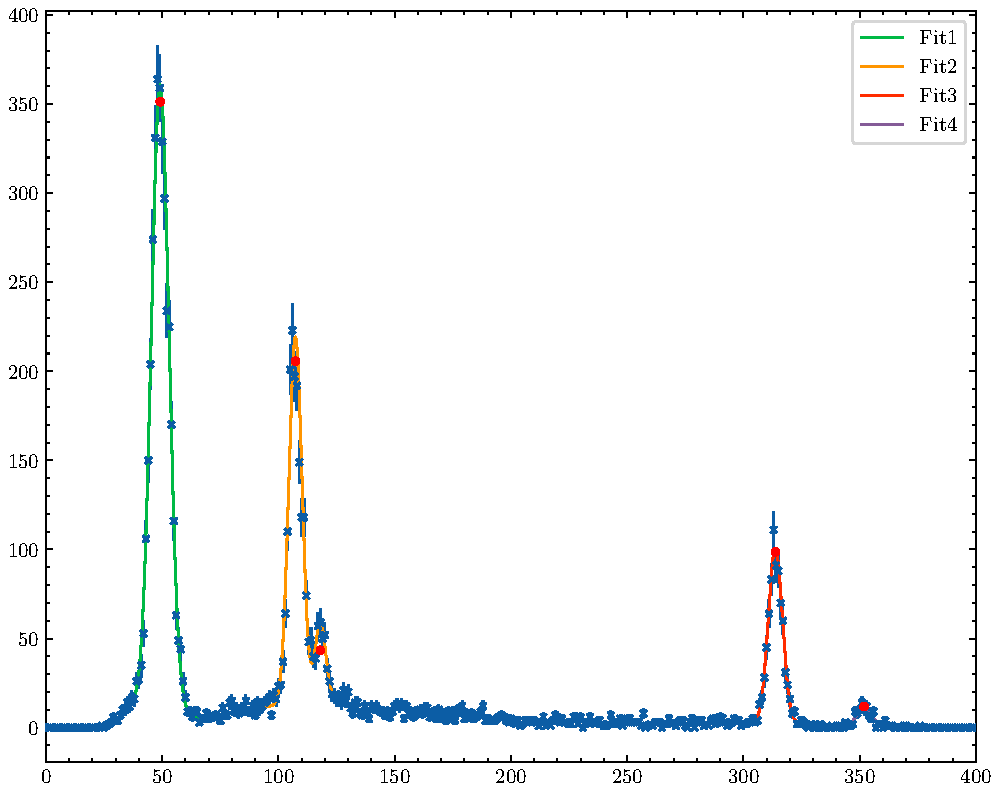
\includegraphics[width=0.6\linewidth]{../figs/In.pdf}
	\caption{Referenzspektrum für Indium.}
	\label{fig:in}
\end{figure}
\begin{figure}[H]
	\centering
	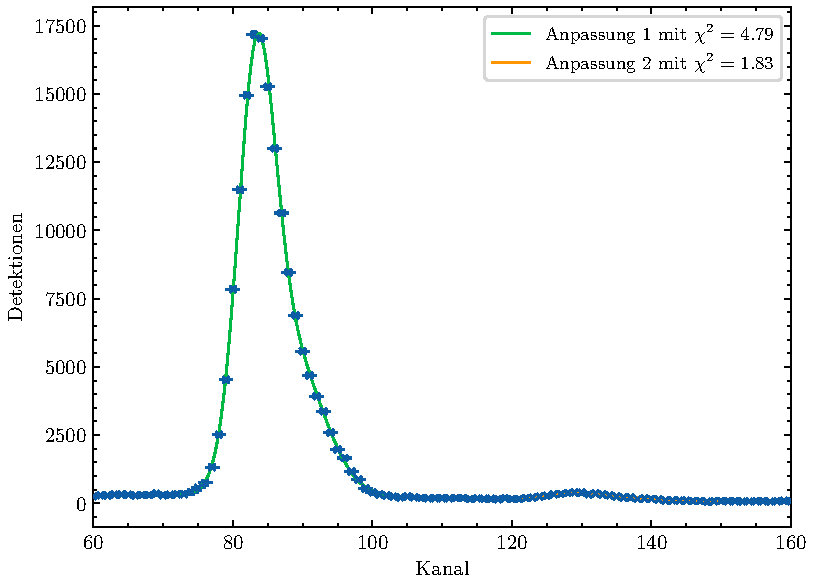
\includegraphics[width=0.6\linewidth]{../figs/Fe.pdf}
	\caption{Referenzspektrum für Eisen.}
	\label{fig:fe}
\end{figure}
\begin{figure}[H]
	\centering
	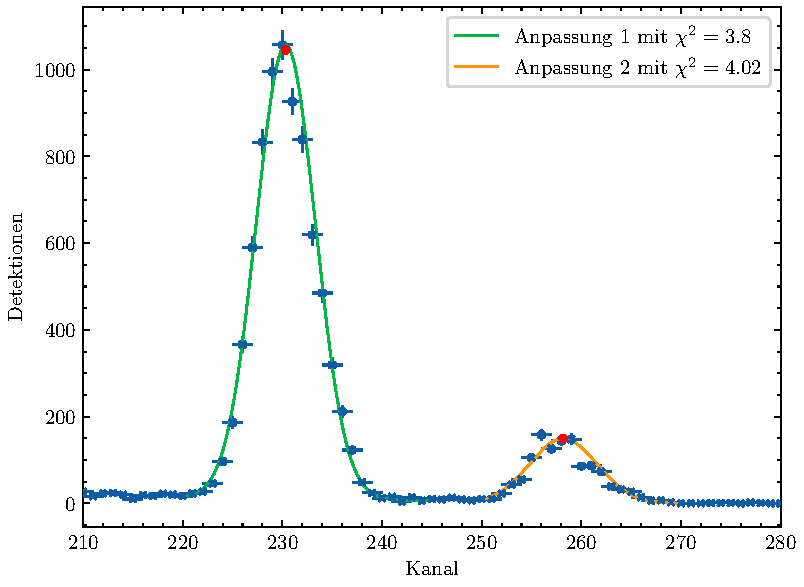
\includegraphics[width=0.6\linewidth]{../figs/Mo.pdf}
	\caption{Referenzspektrum für Molybdän.}
	\label{fig:mo}
\end{figure}
\begin{figure}[H]
	\centering
	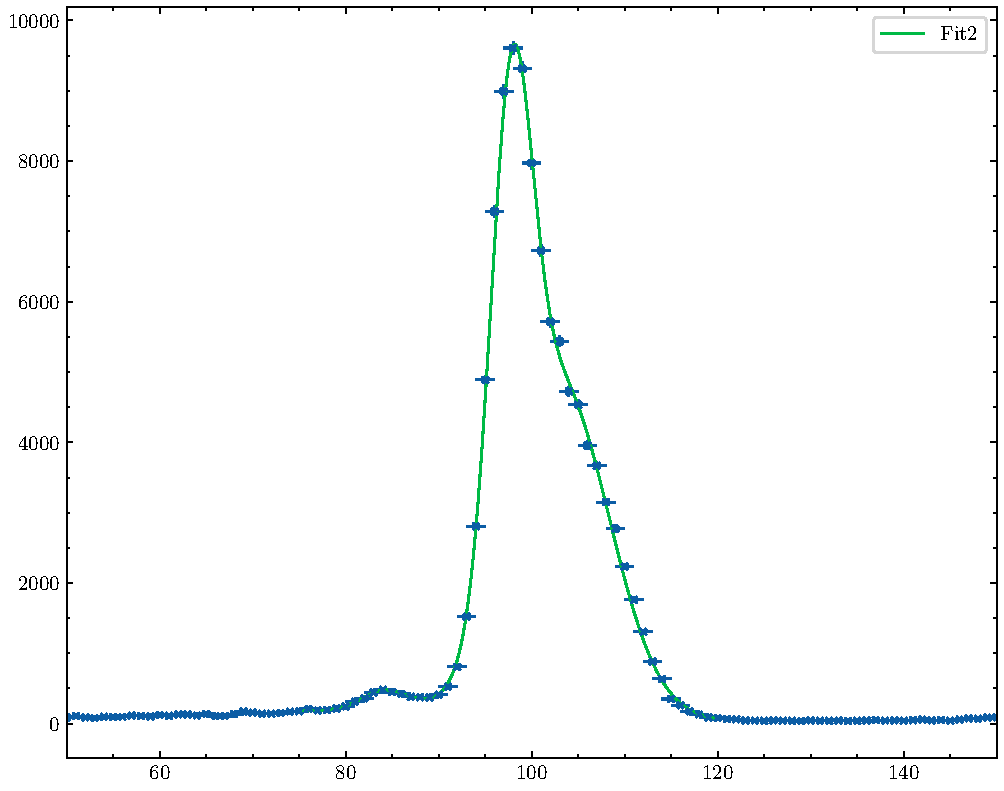
\includegraphics[width=0.6\linewidth]{../figs/Ni.pdf}
	\caption{Referenzspektrum für Nickel.}
	\label{fig:ni}
\end{figure}
\begin{figure}[H]
	\centering
	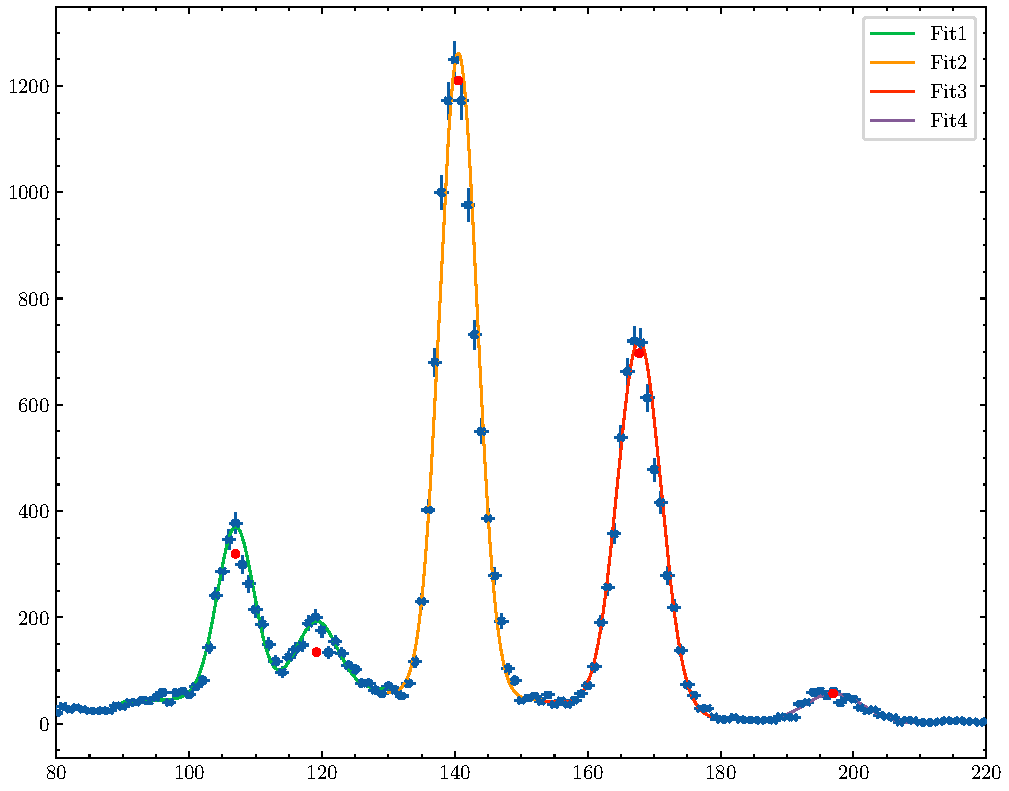
\includegraphics[width=0.6\linewidth]{../figs/Pb.pdf}
	\caption{Referenzspektrum für Blei.}
	\label{fig:pb}
\end{figure}
\begin{figure}[H]
	\centering
	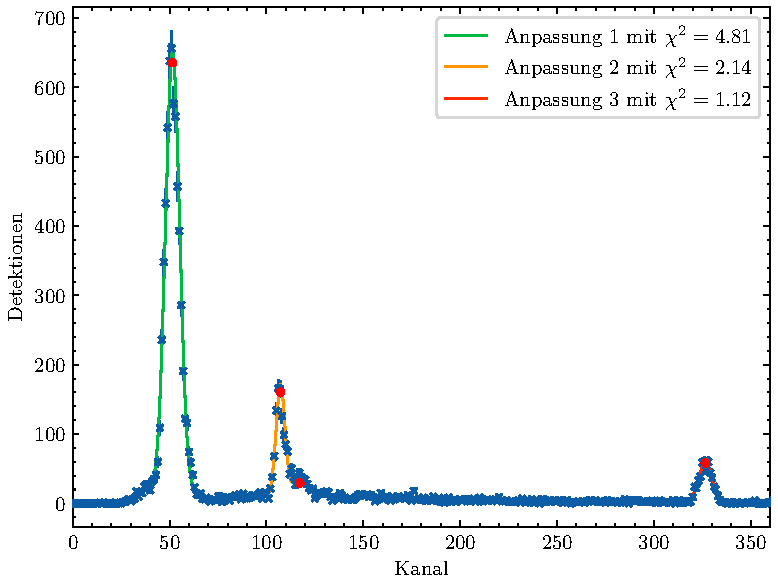
\includegraphics[width=0.6\linewidth]{../figs/Sn.pdf}
	\caption{Referenzspektrum für Zinn.}
	\label{fig:sn}
\end{figure}
\begin{figure}[H]
	\centering
	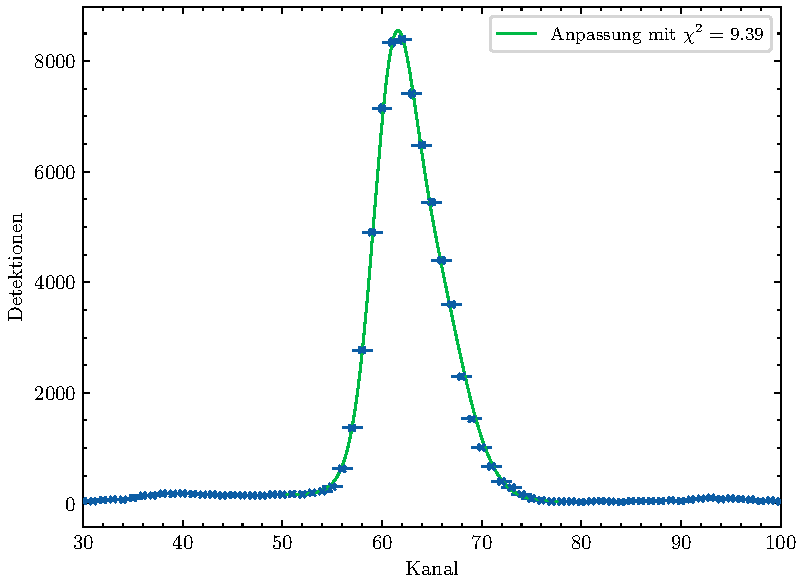
\includegraphics[width=0.6\linewidth]{../figs/Titan.pdf}
	\caption{Referenzspektrum für Titan.}
	\label{fig:ti}
\end{figure}
\begin{figure}[H]
	\centering
	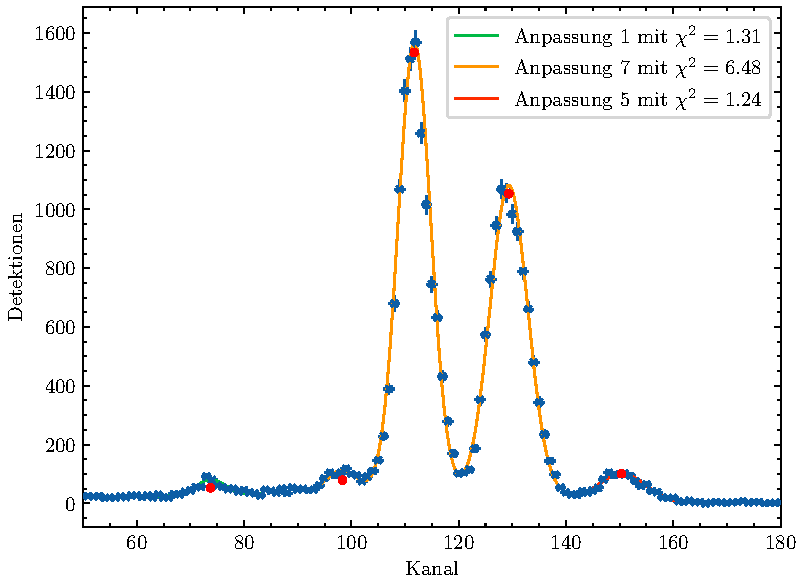
\includegraphics[width=0.6\linewidth]{../figs/W.pdf}
	\caption{Referenzspektrum für Wolfram.}
	\label{fig:w}
\end{figure}
\begin{figure}[H]
	\centering
	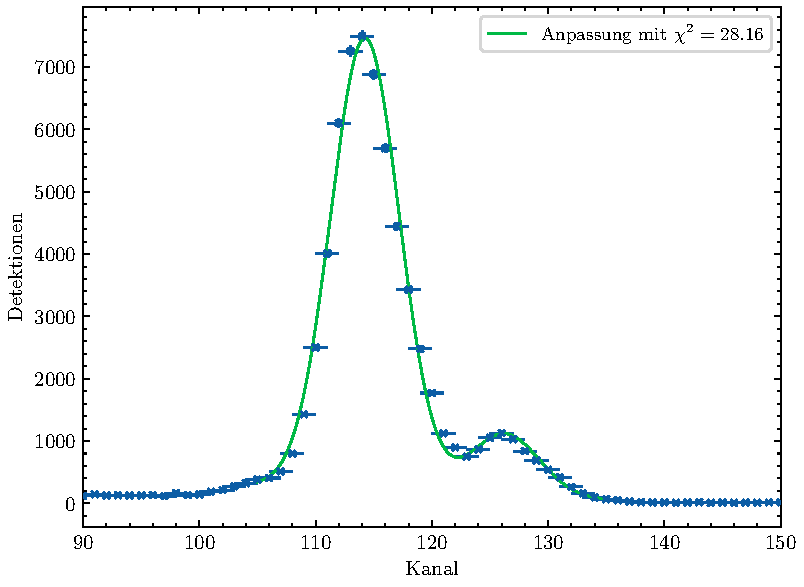
\includegraphics[width=0.6\linewidth]{../figs/Zn.pdf}
	\caption{Referenzspektrum für Zink.}
	\label{fig:zn}
\end{figure}
\begin{figure}[H]
	\centering
	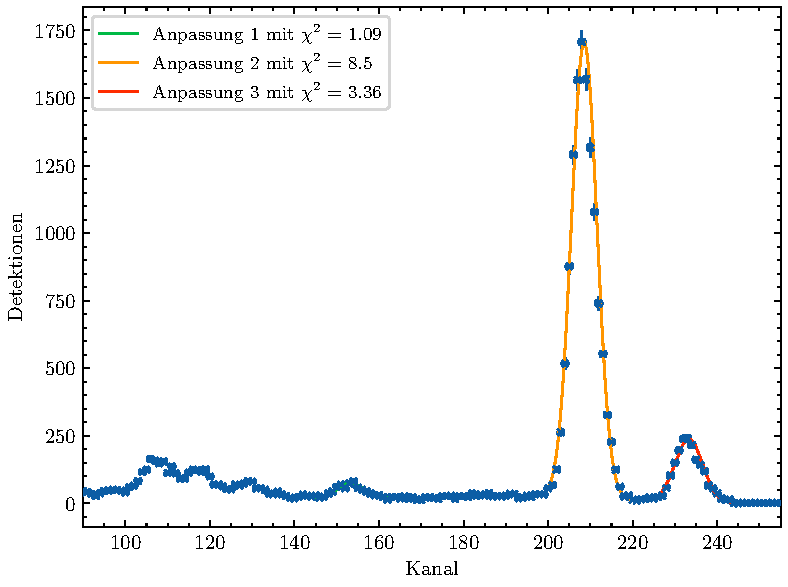
\includegraphics[width=0.6\linewidth]{../figs/Zr.pdf}
	\caption{Referenzspektrum für Zirconium.}
	\label{fig:zr}
\end{figure}